%% cv.tex
%% Copyright 2017 Zeyi Fan
%
% This work may be distributed and/or modified under the
% conditions of the LaTeX Project Public License, either version 1.3
% of this license or (at your option) any later version.
% The latest version of this license is in
%   http://www.latex-project.org/lppl.txt
% and version 1.3 or later is part of all distributions of LaTeX
% version 2005/12/01 or later.
%
% This work has the LPPL maintenance status `maintained'.
%
% The Current Maintainer of this work is Zeyi Fan.
%
% This work consists of only the file cv.tex

\documentclass{article}
\usepackage[top=.4in, bottom=.0in, left=3in, right=0.4in,marginparwidth=2.5in]{geometry}
\usepackage[utf8]{inputenc}
\usepackage{tikz}
\usepackage{xcolor}
\usepackage[absolute,overlay]{textpos}
\usepackage{fontspec}
\usepackage{titlesec}
\usepackage{pstricks}
\usepackage{amssymb}
\usepackage{paralist}

\tolerance=1
\emergencystretch=\maxdimen
\hyphenpenalty=10000
\hbadness=10000

\usepackage[pdfauthor={Cesar Reyes}, pdftitle={Cesar Reyes's Resume}, pdfkeywords={}]{hyperref}
\usepackage{hyperref}

\definecolor{mygray}{gray}{0.95}
\definecolor{lightdark}{gray}{0.55}
\definecolor{dark}{gray}{0.3}
\definecolor{skillbg}{gray}{0.7}

\newcommand{\amount}{5.7in}
\setcounter{section}{-1}

\linespread{1.2}
\pagenumbering{gobble}

\renewcommand{\labelitemi}{$\blacksquare$}
\renewenvironment{itemize}[1]{\begin{compactitem}#1}{\end{compactitem}}

% Helpers
\newcommand\twodigits[1]{%
	\ifnum#1<10 0#1\else #1\fi
}

%\newcommand\hl[1]{{\ralewaysb #1}}
\newcommand\hl[1]{#1}


% Fonts
\newfontfamily\raleway{Raleway}
\newfontfamily\ralewaym{Raleway Medium}
\newfontfamily\ralewaysb{Raleway SemiBold}
\newfontfamily\ralewayb{Raleway Bold}
\newfontfamily\ralewayeb{Raleway ExtraBold}
\newfontfamily\ralewaybb{Raleway Black}

\setmainfont{Raleway}

% Styles
\newcommand{\name}[2]{
	\begin{center}
		\Huge{
			\ralewayeb{#1 #2}
		}
	\end{center}
}

\newcommand{\tagline}[1]{
	\begin{center}
		\large{
			\color{dark}
			\ralewaysb{#1}
		}
		\vspace{.2em}
	\end{center}
}

\renewcommand{\thesection}{\twodigits{\arabic{section}}.}

\titleformat{\section}
[hang]
{\ralewaysb\large\color{dark}}
{}
{.0em}
{}
[{\titlerule[0.8pt]}]

\titlespacing*{\section}{0pt}{4pt}{10pt}

\setlength{\TPHorizModule}{1mm}
\setlength{\TPVertModule}{1mm}
\setlength{\parindent}{0mm}

\newcommand{\contactline}[2]{
	\ralewaysb{#1} & \raleway{#2}
}

\newcommand{\skill}[2]{
	\vspace{.2em}
	\ralewayb{#1}
	
	\psset{xunit=0.197\linewidth, yunit=5pt}
	\begin{pspicture}[showgrid=false](5,1)
	\psline[linecolor=skillbg](0,0.5)(5,0.5)
	\psline[linecolor=skillbg,arrows=|-|](1,0.5)(2,0.5)
	\psline[linecolor=skillbg,arrows=|-|](3,0.5)(4,0.5)
	\psline[linecolor=skillbg,arrows=-|](0,0.5)(5,0.5)
	
	\psline[linecolor=black,arrows=|-|](0,0.5)(#2,0.5)
	\end{pspicture}
}

\newcommand{\block}[3]{
	{\large\ralewayb #1}
	
	\ralewaym{\color{lightdark}#2}
	
	\raleway{#3}
}

\begin{document}
	
	% background
	
	\begin{tikzpicture}[remember picture,overlay]
	\fill[mygray] (current page.south west) rectangle ([xshift=-\amount]current page.north east);
	\end{tikzpicture}
	
	% Side Bar
	
	\begin{textblock}{58.5}(6,7.7)
		    \begin{figure}
		        \centering
		        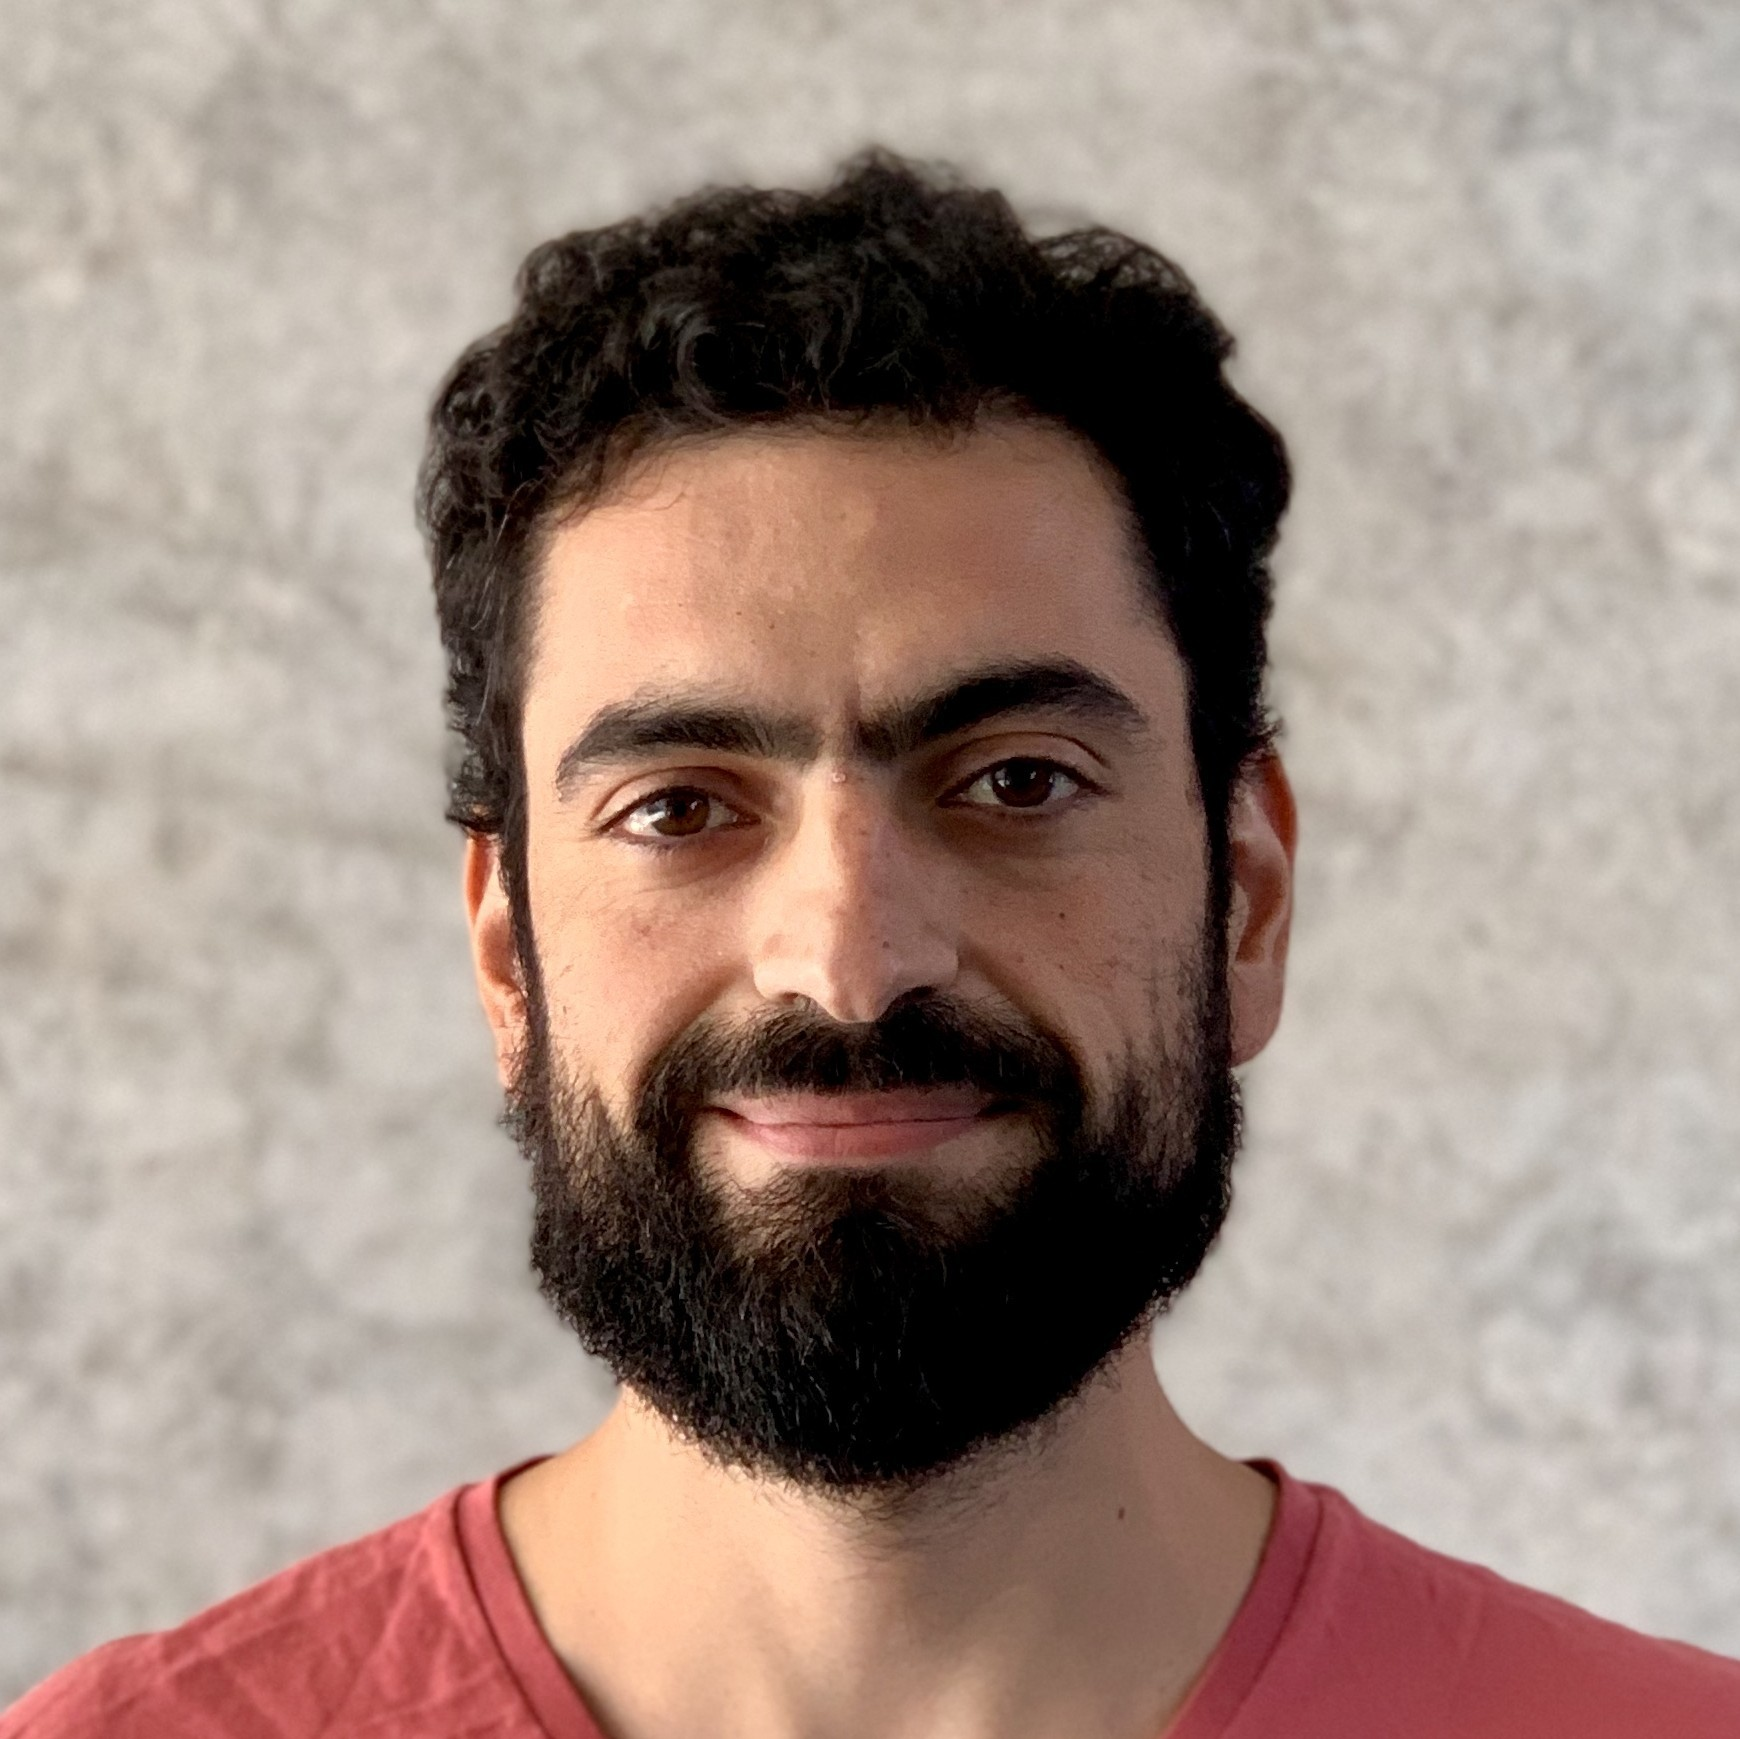
\includegraphics[width=0.8\linewidth]{creyesp.jpg}
		    \end{figure}
		
		\name{C\'esar}{Reyes}
		
		\tagline{Data Scientist \& ML engineer}
		
		\section{Resumen}
		
		\color{dark}
		
		Apasionado en ciencia de datos, inteligencia artificial, y el mundo open source. 
		Autodidacta, difusor del conocimiento, docente y Co-orgaizador de la Meetup de Data Science Montevideo.
		Especial interes en NLP y llevar modelos a producción.
		
		\section{Contacto}
		
		\renewcommand{\arraystretch}{1.1}
		
		\begin{tabular}{rl}
			\contactline{Celular}{(+598) 92716167} \\
			\contactline{Email}{cesar.reyesp@gmail.com} \\
			\contactline{Edad}{32} \\
			\contactline{GitHub}{\href{https://github.com/creyesp}{@creyesp}} \\
			\contactline{LinkedIn}{\href{https://linkedin.com/in/creyesp}{/in/creyesp}}
		\end{tabular}
		
		\section{Habilidades}
		
		%    \skill{Python (+3 años)}{4}
		\textbf{Lenguajes}: Python, R, Bash, Matlab, C/C++\\
		\textbf{Cloud platform}: GCP, Azure CI/CD \\
		\textbf{Stack tecnologico}:  SQL (postgres, mssql), MongoDB, Git, Airflow, Apache Beam, Docker\\
		\textbf{Data analisis}: Numpy, Pandas, Scipy, H5py, Matplotlib, Seaborn, Bokeh,
		Scikit-Learn, TensorFlow, Keras, pytorch, transformers\\
		\textbf{SO}: GNU/Linux
		
		\section{Idiomas}
		\textbf{Español, Ingles}
		
		
	\end{textblock}
	
	% Main
	
	\vspace{-25pt}  % Change this value to adjust the position of the right
	
	\section{Experiencia Laboral}
	\block{Data Scientist}
	{PedidosYa | Montevideo, Uruguay | Mayo 2020 - Actualidad}
	{
		En PedidosYa formó parte del equipo de Analytic Factory el cual brinda apoyo de data analytics en diferentes equipos de producto. Algunas responsabilidades:
		
		\begin{itemize}
			\item Trabajar con los stakeholders identificando oportunidad y mejoras en los productos usando técnicas de ML.
			\item Desarrollar modelos de ML y llevar estos a producción (GCP).
			\item Uso de transformers para detection de topicos en chat de usuarios basados en la semantica.
			\item Desarrollar framework para realizar A/B testing
		\end{itemize}
	}
	
	\vspace{.5em}
	
	\block{Docente}
	{Universidad ORT | Montevideo, Uruguay | Octubre 2020 - Actualidad}
	{
		Docente de la materia Machine Learning Supervisado en el Diploma de Especialización en Analítica de Negocios con foco en modelos en R.
		
	}
	
	\vspace{.5em}
	
	
	\block{Data Scientist/ML Engineer}
	{Alphalabs | Montevideo, Uruguay | Junio 2020 - Actualidad}
	{
		Co-fundador de AlphaLabs y miembro del área de Data Science. Mis responsabilidades son:
		
		\begin{itemize}
			\item Implementación de modelos de ML y ETL en streaming de datos (GCP).
			\item Uso de técnicas de scraping para recolección de data disponible en internet.
			\item Desarrollo de APIs para disponibilizar modelos (GCP).
			\item Deploy de un modelo basado en Bert usando torchserve (GCP).
		\end{itemize}
		
	}
	
	\vspace{.5em}
	
	\block{Data Scientist}
	{Bluekiri | Montevideo, Uruguay | Enero 2019 - Mayo 2020}
	{
		Bluekiri parte del grupo Logitravel (rubro del turismo) donde el área de Data Science presta servicios a las líneas de negocio para descubrir e impulsar las decisiones basadas en datos. Mis responsabilidades eran:
		
		
		\begin{itemize}
			\item Desarrollar un modelo de recomendación de precio para hoteles y un modelo de predicción de cancelación de reservas.
			\item Analizar data interna de la empresa para dar insights accionables a negocio.
			\item Desarrollo de bibliotecas custom en Python (CI/CD) para manejar desde la colección de los dato, el modelado hasta el reporte de los proyectos
			\item Automatiza pipelines de datos con Apache Airflow
			\item Uso de diversos servicios de Google Cloud y Azure CI/CD.
		\end{itemize}
		
	}
	
	
	\vspace{.5em}
	
	\block{Data Scientist}
	{Universidad Técnica Federico Santa María | Remoto | Mayo 2018 – Diciembre 2018 }
	{
		En el marco de un proyecto de Neurociencia en colaboración del el Instituto de Sistemas Complejos de Valparaíso y la UTFSM formaba parte de un equipo que está contribuir en el campo científico. Mis responsabilidades eran:
		
		\begin{itemize}
			\item Recolectar la data, realizar exploración, análisis y visualización de estos.
			\item Desarrollo del package Spikelib alojado en PyPi.
			\item Desarrollo e implementación de templates para el análisis y procesamiento de datos.
			\item Generación de modelos estadísticos.
			\item Generación de reportes periódicos.
		\end{itemize}
		
	}
	
	\vspace{.5em}
	\newpage

	\block{Research Assistant}
	{Universidad Técnica Federico Santa María | Valparaíso, Chile | Abril 2015 – Febrero 2018}
	{
		Integrante de un proyecto de investigación de neurociencia donde junto a un equipo multidisciplinarios trabajamos en descubrir el funcionamiento del sistema visual. 
		
		Publicaciones: \\
		Characterization of Retinal Functionality at different Eccentricities in a Diurnal Rodent \url{https://doi.org/10.1101/277814 }
	}
	
	\vspace{.5em}

	
	\block{Software developer}
	{Centro Interdisciplinario de Neurociencia Valparaíso | Valparaíso, Chile | Marzo 2017 – Febrero 2018}
	
	\vspace{.5em}
	\section{Educación}
	
	\block{Ingeniero Civil Electrónico con especialidad en Informática}
	{Universidad Técnica Federico Santa María - Titulado 2016}
	{
		Memoria de título profesional: Creación de un módulo en Snort para la detección de intrusos en la red con técnicas estadísticas. Desarrollado en C.
		
	}
	
	\section{Pasantías}
	\block{Pasantia Universitaria}
	{Altavoz S.A.  | Viña del Mar, Chile | Marzo 2014 – Abril 2014}

	
	\block{Pasantia Universitaria}
	{Axiovista S.A.   | Santiago, Chile | Enero 2013 – Febrero 2013}
	
	\section{Cursos}
	\begin{itemize}[-]
		\item Deploy Machine learning Model in Production (udemy) \hfill 2020
		\item Full Stack Deep Learning Course \hfill 2020
		\item Hands-On Machine Learning with Scikit-Learn, Keras, and TensorFlow, (book) 2nd Edition \hfill 2020
		\item The Hundred-Page Machine Learning Book (book) by Andriy Burkov \hfill 2019   

		\item Workshop Categorización de Productos con Deep Learning (Mercado Libre) \hfill 2019
		\item PyData Córdoba \hfill 2019
		\item Curso online de data science en python dictado por la Universidad de San Diego, California por el portal EdX (Python for Data Science UCSanDiegoX - DSE200x). \hfill 2018
		\item  Workshop dictado por Tryolabs para la detección de objetos usando TensorFlow.  \hfill Nov 2018

	\end{itemize}

	\section{Reconocimientos}
	
	\ralewaysb Excelencia Académica. \raleway Universidad Técnica Federico Santa María \hfill 2007-2012
	\ralewaysb Mérito Académico. \raleway Departamento de Electrónica - UTFSM\hfill 2007
	
	\section{Otras actividades}
	Co-Organizado de la Meetup Montevideo Applied Data Science and Big Data UY


\end{document}
